%%%%%%%%%%%%%%%%%%%%%%%%%%%%%%%%%%%%%%%%%%%%%%%%%%%%%%%%%%%%%%%%%%%%%%
% writeLaTeX Example: Academic Paper Template
%
% Source: http://www.writelatex.com
%
% Feel free to distribute this example, but please keep the referral
% to writelatex.com
%
%%%%%%%%%%%%%%%%%%%%%%%%%%%%%%%%%%%%%%%%%%%%%%%%%%%%%%%%%%%%%%%%%%%%%%
% How to use writeLaTeX:
%
% You edit the source code here on the left, and the preview on the
% right shows you the result within a few seconds.
%
% Bookmark this page and share the URL with your co-authors. They can
% edit at the same time!
%
% You can upload figures, bibliographies, custom classes and
% styles using the files menu.
%
% If you're new to LaTeX, the wikibook is a great place to start:
% http://en.wikibooks.org/wiki/LaTeX
%
%%%%%%%%%%%%%%%%%%%%%%%%%%%%%%%%%%%%%%%%%%%%%%%%%%%%%%%%%%%%%%%%%%%%%%
\documentclass[twocolumn,showpacs,%
  nofootinbib,aps,%superscriptaddress,
  eqsecnum,prd,notitlepage,showkeys,10pt]{revtex4-1}

\usepackage{amssymb}
\usepackage{amsmath}
\usepackage{graphicx}
\usepackage{dcolumn}
\usepackage{threeparttable}
\usepackage{algorithm}
\usepackage{algpseudocode}
\usepackage[hidelinks]{hyperref}
\usepackage[T1]{fontenc}
\usepackage{array}
\usepackage{makecell}
\newcolumntype{x}[1]{>{\centering\arraybackslash}p{#1}}
\usepackage{tikz}
\usepackage{pgfplots}

% table thick line
\makeatletter
\newcommand{\thickhline}{%
    \noalign {\ifnum 0=`}\fi \hrule height 1pt
    \futurelet \reserved@a \@xhline
}

\newcommand\diag[4]{%
  \multicolumn{1}{p{#2}|}{\hskip-\tabcolsep
  $\vcenter{\begin{tikzpicture}[baseline=0,anchor=south west,inner sep=#1]
  \path[use as bounding box] (0,0) rectangle (#2+2\tabcolsep,\baselineskip);
  \node[minimum width={#2+2\tabcolsep-\pgflinewidth},
        minimum  height=\baselineskip+\extrarowheight-\pgflinewidth] (box) {};
  \draw[line cap=round] (box.north west) -- (box.south east);
  \node[anchor=south west] at (box.south west) {#3};
  \node[anchor=north east] at (box.north east) {#4};
 \end{tikzpicture}}$\hskip-\tabcolsep}}


\begin{document}

\title{Practical Application of Web-Based Authentication using Keystroke Dynamics}

\author{Yuankai Guo}
\email{u0942867@utah.edu}
\affiliation{University of Utah}
\author{Myungho Jung}
\email{myungho.jung@utah.edu}
\affiliation{University of Utah}
\author{Junwei Shi}
\email{sjwarthas2009@gmail.com}
\affiliation{University of Utah}
\author{Xu Wang}
\email{xu724@cs.utah.edu}
\affiliation{University of Utah}

%\begin{abstract}
%Keystroke dynamics has been studied for many years and proved that each user's keystroke pattern is unique. Through the project, we developed a login application to authenticate users by comparing keystroke patterns. We also %tested possible variation of patterns on controlled environment. Unlike other studies, we considered how to apply the mechanism to existing web services.
%\end{abstract}

\maketitle

\section{Introduction}
Password authentication has been one of the most popular method to identify. However, attackers' techniques to steal password have also been developed in many ways. Therefore, we need different methods to figure out identity other than just plain text of passwords. For example, access from different IP or MAC address can be detected as a suspicious behavior or attack. However, most of the additional authentication algorithms make users inconvenient. Keystroke dynamics can be extracted while typing password as well as used as identity verification\cite{gaines1980authentication}. We will show that the existing users don't have to buy an additional device as well as only a small change in the existing servers will be required to apply it.

\section{Related Works}
Many algorithms to detect outliers were studied and tested on performance and precision\cite{shanmugapriya2009survey}. Various algorithms were used for pattern matching, such as neural network, Support Vector Machines, K-Nearest Neighbors, and Euclidean distance. For most researches, hundreds of patterns from dozens of people were collected and tested. On the other hand, we focused on comparing the performance of algorithms depending on the variation of the users. One of the defects of the result from most existing tests is that they intentionally collected data from a certain group of people. If the group only consisted of experienced users, the data would be biased. Also, the variation of patterns cannot be observed in a short period of data. We formulated a hypothesis on three changes in patterns and tested in well-controlled environment.

\section{Threat Model}
Id and password login system is ubiquitous for identification on the internet. However, as the number of web services has dramatically increased, it becomes impossible for people to remember many different passwords and most of them are using the same password for all web sites. It would be a problem if a cracker breaks in a insecure server and steals users' passwords, the password can be used for other web services as well.
\par
On the other hand, keystroke dynamics is one of the biometric authentication such as face, fingerprint, and iris recognition\cite{karnan2011biometric}. Thus, past data become naturally useless for authentication. Also, a set of patterns can be stores as a different form of structure like a neural network. It makes hard for attackers to imitate the keystroke pattern.

\section{Method}
\subsection{Data structure}
\begin{figure}[h]
  \centering
  \includegraphics[width=0.4\textwidth]{keystroke}
  \caption{Timing measurement in interval and duration}
  \label{fig:keystroke}
\end{figure}

The timing vector of keystroke patterns can be measured as intervals between keys and keystroke durations\cite{cho2000web}. Therefore, given $n$ characters password, a pattern is represented as an array of $n+1$ numbers. We applied the structure in a slightly different way from other studies. The interval in our project was measured not from previous release time but from press time. By doing so, there is no negative value and storage can be saved by storing only unsigned data. The timing vector can be considered as a point in $n+1$ dimensional space. Then, we can compare similarity using statistical or machine learning algorithms.
\par
The pattern needs to be normalized because the storage is limited and in order to equivalent comparison among users. First, the timing values were divided by the maximum value and stored with the maximum value. Then, the values becomes less than 1 and the data size can be controlled by floating point precision. Also, two different length of passwords cannot be evaluated with the same error bound because of different dimensional space. we solved the problem by multiplying the error bound by $\sqrt{d}$ such that $d$ is the order of dimension.

\subsection{Algorithm}
To filter imposter's patterns, novelty detection algorithms are required. There are many researches to detect anomaly\cite{banerjee2012biometric}. We selected and tested three common algorithms, which are the Nearest Neighbor, Mahalanobis distance, and one class SVMs, with changing the patterns.

\section{Implementation}
\subsection{Architecture}
Our system is built based on the B/S model. We use an HTML page as the frontend and program a series of Python sciprts as the backend. The frontend collects the timing pattern from the user and send it with encryption to the backend via AJAX. The backend retrieve previously stored feature pattern from a database and match it against the input with our novelty detection algorithm. If the matching is successful, a positive result is send to the frontend, and vice versa.
\par
A user's inputting habit may change over time. Therefore, we need to regenerate the feature pattern periodically. Every time the authentication is successful, we record the timing pattern from the user into database. And when a certain number of patterns are collected. We run the training routine of our novelty detection algorithm to generate a new feature pattern.

\subsection{Encryption}
It's not secure to transmit the password and pattern in plaintext through the network. So we need to protect the password and pattern by encryption or message digest. In our implementation, we use one handshake protocol instead of multiple handshakes for better efficiency. The format of authentication message is $Key{Hash(TS|Pattern)|TS|Pattern}$ such that $TS$ is timestamp. The $Key$ is 128bit generated from $MD5$ message digest of password. We generate $Hash(TS|Pattern)$ using $SHA-1$, which provides integrity protection for the message. We encrypt the $Hash(TS|Pattern)|TS|Pattern$ by $AES$ algorithm. Moreover, we add a salt to for better diversity. With the timestamp and salt, it's invulnerable to rainbow attack.
\par
How to prevent replay attack? In our implementation, the server record the timestamp. If the server receives a message with the same timestamp which already exists in the time window, the server will refuse the message. Of course, the server will also drop the message with invalid timestamp.
\par
However, there is a drawback in the protocol. Since the client couldn't authenticate the identity of the server, it's vulnerable to in-the-middle attack. Besides, the protocol is not secure when it comes to server break-in attack. The attacker could also modify the time in the server.

\section{Analysis}
 We created a pattern generator to test algorithms. Our tests are focused on the prediction of the variation of user's patterns and comparing performances of pattern matching methods. The error rates for pattern detection are divided into two parts which are False Acceptance Rate(FAR) and False Rejection Rate(FRR)\cite{cho2000web}. The two error rates are calculated for each test case.

\subsection{Environment}
Test program is coded in python using Scipy, Numpy, and scikit-learn library. For each test, 1000 evenly distributed patterns of imposters are generated. Also, the same number of patterns of the Gaussian distribution for genuine users are created. If our assumption is correct, the distribution of patterns will be similar to actual patterns from a user and imposters.
\par
Our tests are focused on the variation of the patterns over time. First, only an interval of patterns would be fluctuated. Suppose that the password is mixed with a sequence of alphabets and that of numbers like `foo1234.' In this cases, the patterns of a word and numbers may be stable except the interval between them. Second, we assume that the user will type the password fast or slow; however, the pattern would be proportional. The third assumption is that the user may use different types of keyboards such as laptop, desktop keyboard, and touch keyboard on mobile devices. Then, we expected that the patterns will form multiple clusters.

\subsubsection{Test Results}
\begin{figure}[ht]
  \centering
  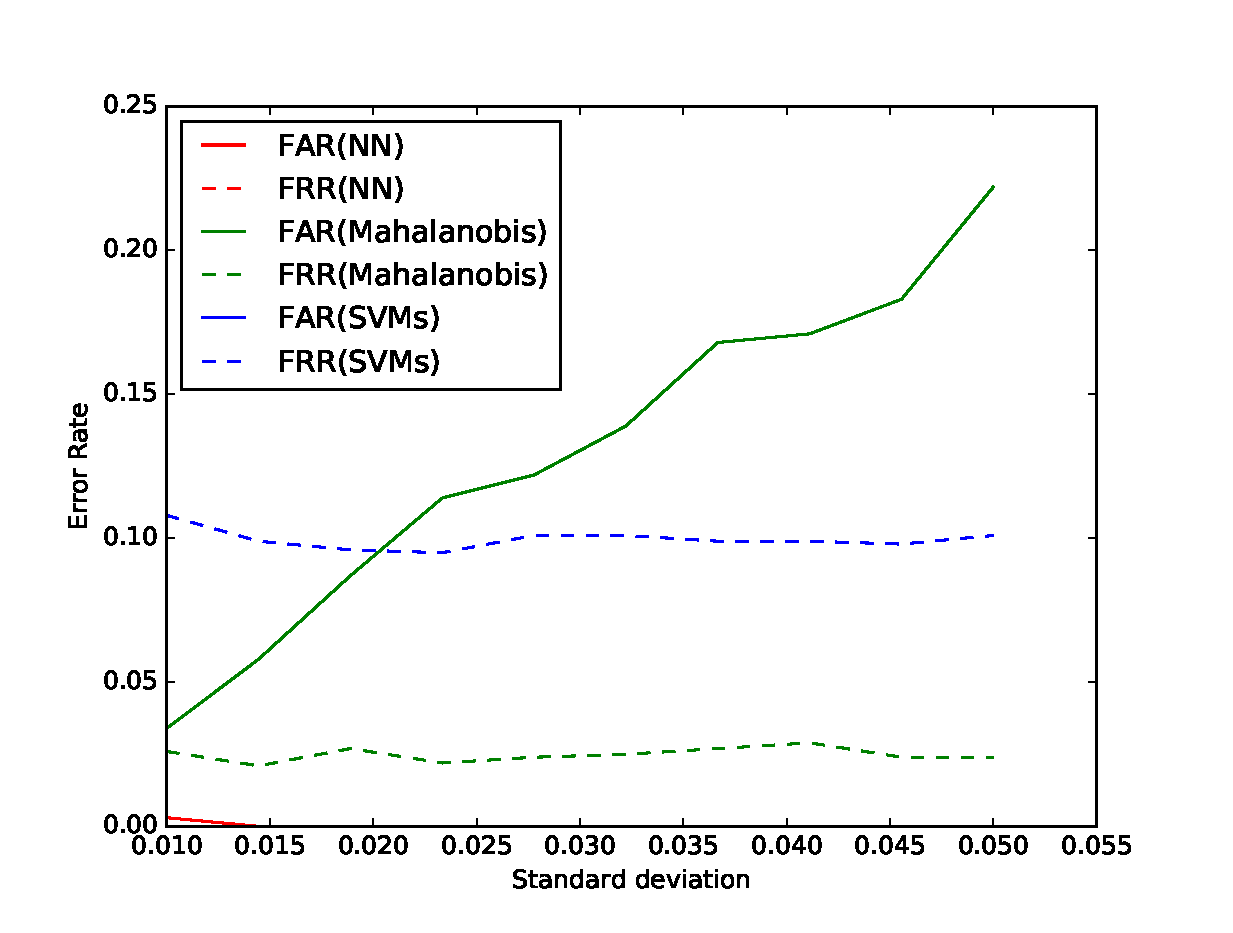
\includegraphics[width=0.44\textwidth]{one}
  \caption{Test result of patterns that only one of the intervals varies}
  \label{fig:one}
\end{figure}
\begin{figure}[ht]
  \centering
  \includegraphics[width=0.44\textwidth]{prop}
  \caption{Test result of proportional patterns}
  \label{fig:prop}
\end{figure}
\begin{figure}[ht]
  \centering
  \includegraphics[width=0.44\textwidth]{multi}
  \caption{Test result of patterns of multiple clusters}
  \label{fig:multi}
\end{figure}

Most of the error rates are not visible because they are very close to 0. As seen in the three tests, we concluded that the performances of the three algorithms are not much different regardless of the variation of the patterns. The most accurate method among them was the nearest neighbor method, the SVMs was next, and the Mahalanobis distance showed the worst performance. With respect to computation time, the SVMs was the fastest, the nearest neighbor was next, and the Mahalanobis distance was the slowest. However, the difference in performance may come from different libraries used. The SVMs and nearest neighbor using ball tree algorithm were implemented using $scikit-learn$ library. On the other hand the Mahalanobis distance was measured using $scipy$ library.

\section{Defects}
Although many researches and practical application of Keyboard Dynamics exist, there are problems in keystroke authentication. Assume that the mechanism is applied for Web-based system. Then, people can move cursors using arrow keys or mouse while typing and editing password. We just ignored the cases and assumed that the web page allows only password typed at once. Though it would make the users inconvenient, it will make the system more secure. Also, key stroke patterns may be able to be recorded by spyware with key logger. In general, we don't have to worry about the attack because the pattern is encrypted before sent. If the encryption cannot be applied on the system, it can be protected by the attack by sharing a nonce with the server and adding it to the pattern. lastly, a user's patterns change more frequently and radically than other physiological traits or behavioral characteristics, and thus it would be a problem. We suggest a solution that evaluates only the latest patterns like sliding window.

\section{Conclusion}
Through the project, we checked the algorithm is valid by demo program and also tested the performance between algorithms. We suggested that the possible web-based authentication using keystroke dynamics by implementing and testing actual login web page. Unfortunately, it is not obvious that the test data is significant compared to that from other research. However, the application developed for the experiments will be useful to test other algorithms with a myriad of normally distributed patterns and variations. It will help to create various environments for next experiments.

%%%%%%%%%% BIBLIOGRAPHY %%%%%%%%%%
\bibliographystyle{plain}
\bibliography{report}

\end{document}
